\documentclass{beamer}
\usetheme{metropolis}
%%%
\usepackage{polyglossia}
\setmainlanguage{spanish}
\setotherlanguages{english}
%%%
\usepackage{url}
\usepackage{lscape}
\usepackage[squaren]{SIunits}
\usepackage{spverbatim}
%%% 
\usepackage{csquotes}
\usepackage[style=authoryear-comp, backend=bibtex]{biblatex} 
% \bibliographystyle{plainnatR} 
% backend=biber  % for biber
% apalike harvard chicago unsrtnat elsart-num-names
% \bibliography{referencias}
\addbibresource{referencias.bib}
%%%
% R/knitr
\usepackage{tikz}
\usepackage{rotating}
\usepackage{subfig}
\usepackage{inconsolata}
\usepackage{dcolumn}   % requerido por stargazer y texreg
\usepackage{booktabs}  % requerido por xtable y texreg
%%%
\usepackage{syntonly}
%\syntaxonly %verifica sintaxis sin generar documento
%%%

%%%%%%%%%%%%%%%%%% hipervinculos activos %%%%%%%%%%%%%%%%%%%%%%%

% \ifx\pdfoutput\undefined % We're not running pdftex
% \RequirePackage[bookmarks,hyperindex,plainpages=false]{hyperref}
% %colorlinks,
% \else
% \RequirePackage[bookmarks,hyperindex,plainpages=false]{hyperref}
% \def\pdfBorderAttrs{/Border [0 0 0] } % No border arround Links
% \hypersetup{pdfauthor={Ulises M. Alvarez}}
% \hypersetup{pdftitle={Sophie UNAM}}
% \fi
%%%%%%%%%%%%%%%%%%

\title{Git II - GitHub desde la consola}
% Use metropolis theme
\date{Junio 2017}

\author{Ulises M. Alvarez\\ %
%   Proyecto Sophie UNAM\\ %
   $<$\href{mailto:uma@sophie.unam.mx}% 
   {uma@sophie.unam.mx}$>$
}

\institute{Sophie UNAM}

\begin{document}

\maketitle

% \begin{frame}{Brevario}
%   \setbeamertemplate{section in toc}[sections numbered]
%   \tableofcontents[hideallsubsections]
% \end{frame}

% \section{Caracter\'isticas a considerar}
% \label{sec:caracteristicas}

\begin{frame}
  \frametitle{GitHub}
  \begin{itemize}
  \item Es un sistema de control de versiones basado en Git y,
    simult\'aneamente, un servicio de alojamiento.
  \item Ofrece control de cambios y administraci\'on de c\'odigo
    fuente.
  \item Provee control de accesos, seguimiento de errores, peticiones
    de funcionalidad, administraci\'on de tareas y \textit{wikis.}
  \item Permite acceso v\'\i{}a \texttt{ssh.}
  \end{itemize}
\end{frame}

\begin{frame}[standout]
  GitHub vía ssh
\end{frame}

\begin{frame}[fragile]
  \frametitle{GitHub vía ssh}
  El uso del protocolo, \texttt{ssh}, permite conectarse a \textit{GitHub}
  sin tener que proporcionar el usuario y contrase\~na. Pero es necesario
  generar \emph{llaves} de intercambio seguras.
\end{frame}

\begin{frame}[fragile]
  \frametitle{I. Verificar llaves}
  Antes de generar llaves SSH, es necesario verificar si existen:
\begin{verbatim}
$ ls -al ~/.ssh
total 80
.
..
authorized_keys
id_rsa
id_rsa.pub
known_hosts
\end{verbatim}
\end{frame}

\begin{frame}[fragile]
  \frametitle{I. Verificar llaves}
  \begin{itemize}
  \item Si no tiene llaves disponibles, o si desea usar un nuevo par para
    conectarse a \textit{GitHub}, tendr\'a{} que generarlo.
  \end{itemize}
\end{frame}

\begin{frame}[fragile]
  \frametitle{II. Generar llaves SSH}
  Ejecute el siguiente comando desde su terminal:
\begin{verbatim}
$ ssh-keygen -t rsa -b 4096 -C "your_email@example.com"
\end{verbatim}
  \begin{itemize}
  \item Cuando se le pregunte por el archivo donde guardar las llaves,
    presione \texttt{Enter}.
  \item Ingrese la \emph{frase de protecci\'on.}
  \end{itemize}
\end{frame}

\begin{frame}[fragile,fragile]
  \frametitle{III. Agregar llaves a ssh-agent}
  1. Inicie \texttt{ssh-agent} en la terminal:
\begin{verbatim}
$ eval "$(ssh-agent -s)"
\end{verbatim}
  2. Agregue la llave mediante:
\begin{verbatim}
$ ssh-add ~/.ssh/id_rsa
\end{verbatim}
  \begin{itemize}
  \item Reemplace, \emph{id\_rsa}, con el nombre de la llave generada
    anteriormente.
  \end{itemize}
\end{frame}

\begin{frame}[fragile]
  \frametitle{IV. Agregar llave a GitHub}
  1. Copie la llave p\'ublica al portapapeles:
\begin{verbatim}
$ xclip -sel clip < ~/.ssh/id_rsa.pub
\end{verbatim}
\end{frame}

\begin{frame}[fragile]
  \frametitle{IV. Agregar llave a GitHub}
  2. Vaya a su perfil de \textit{GitHub} y abra los ajustes:
  \begin{figure}[hp]
    \centering 
\includegraphics[width=0.4\textwidth]{fig/userbar-account-settings}
    % \caption{Creando un nuevo repositorio.}
    \label{fig:gssh01}
  \end{figure}
\end{frame}

\begin{frame}[fragile]
  \frametitle{IV. Agregar llave a GitHub}
  3. Haga clic sobre el apartado \textbf{Llaves SSH GPG}:
  \begin{figure}[hp]
    \centering 
\includegraphics[width=0.4\textwidth]{fig/settings-sidebar-ssh-keys}
    % \caption{Creando un nuevo repositorio.}
    \label{fig:gssh02}
  \end{figure}
\end{frame}

\begin{frame}[fragile]
  \frametitle{IV. Agregar llave a GitHub}
  4. Vaya a \textbf{Nueva llave SSH}:
  \begin{figure}[hp]
    \centering 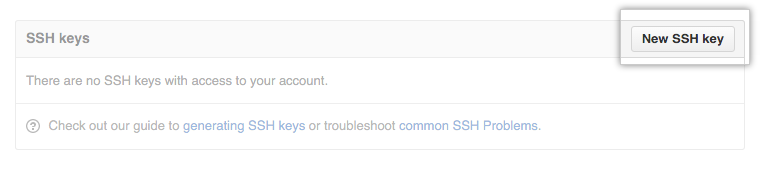
\includegraphics[width=0.75\textwidth]{fig/ssh-add-ssh-key}
    % \caption{Creando un nuevo repositorio.}
    \label{fig:gssh03}
  \end{figure}
\end{frame}

\begin{frame}[fragile]
  \frametitle{IV. Agregar llave a GitHub}
  \begin{itemize}
  \item[5.] Agregue un t\'\i{}tulo descriptivo.
  \item[6.] Pegue la llave p\'ublica en el campo respectivo.
  \end{itemize}
  \begin{figure}[hp]
    \centering 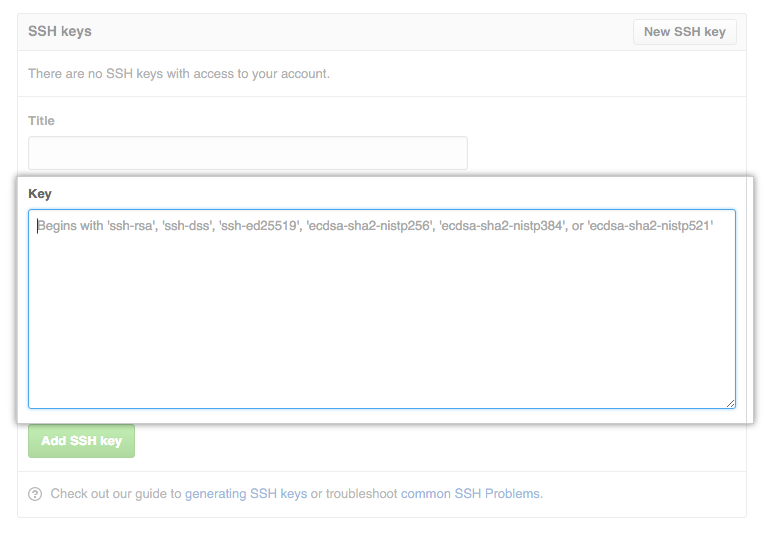
\includegraphics[width=0.6\textwidth]{fig/ssh-key-paste}
    % \caption{Creando un nuevo repositorio.}
    \label{fig:gssh04}
  \end{figure}
\end{frame}

\begin{frame}[fragile]
  \frametitle{IV. Agregar llave a GitHub}
  7. Agregue la nueva llave:
  \begin{figure}[hp]
    \centering 
\includegraphics[width=0.4\textwidth]{fig/ssh-add-key}
    % \caption{Creando un nuevo repositorio.}
    \label{fig:gssh05}
  \end{figure}
\end{frame}

\begin{frame}[fragile]
  \frametitle{IV. Agregar llave a GitHub}
  8. De ser necesario, Ingrese su contrase\~na de \textit{GitHub:}
  \begin{figure}[hp]
    \centering 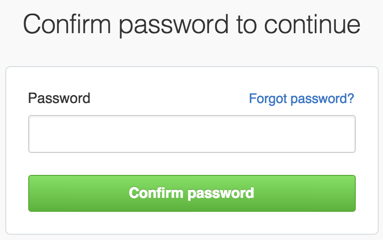
\includegraphics[width=0.4\textwidth]{fig/sudo_mode_popup}
    % \caption{Creando un nuevo repositorio.}
    \label{fig:gssh06}
  \end{figure}
\end{frame}

\begin{frame}[standout]
  Subir un repositorio local
\end{frame}

\begin{frame}[fragile]
  \frametitle{Subir repositorio - CLI}
  \begin{figure}[hp]
    \centering 
\includegraphics[width=0.75\textwidth]{fig/new-project-cli}
    \caption{\href{https://help.github.com/articles/adding-an-existing-project-to-github-using-the-command-line/}%
      {C\'omo subir nuevo repositorio desde CLI.}}
    \label{fig:ghcli}
  \end{figure}
\end{frame}

\begin{frame}[standout]
  Para saber m\'as
\end{frame}

\begin{frame}[fragile]
  \frametitle{Para saber m\'as}
  \begin{itemize}
  \item \href{https://help.github.com/articles/connecting-to-github-with-ssh/}%
    {Connecting to GitHub with SSH}
  \item \href{https://help.github.com/articles/checking-for-existing-ssh-keys/}%
    {Checking for existing SSH keys}
  \item \href{https://help.github.com/articles/generating-a-new-ssh-key-and-adding-it-to-the-ssh-agent/}%
    {Generating a new SSH key and adding it to the ssh-agent}
  \item \href{https://help.github.com/articles/adding-a-new-ssh-key-to-your-github-account/}%
    {Adding a new SSH key to your GitHub account}
  \item \href{https://help.github.com/articles/adding-an-existing-project-to-github-using-the-command-line/}%
    {Adding an existing project to GitHub using the command line}
  \end{itemize}
\end{frame}

% % \section{Conclusiones}
% % \label{sec:conlusiones}


% \begin{frame}[standout]
%   Qué lenguaje usar
% \end{frame}

% \begin{frame}{Conclusiones}
%   \begin{itemize}
%   \item Lo que use mi gremio (\emph{siempre y cuando sea de código
%     abierto}).
%   \item El que se integre mejor a mi flujo de trabajo.
%   \item Perspectiva de desarrollo académico (\emph{no siempre el más
%     usado es el mejor}).
%   \end{itemize}
% \end{frame}


\end{document}
%%% Local Variables:
%%% mode: latex
%%% mode: flyspell
%%% TeX-engine: xetex
%%% End:
